\documentclass[11pt,a4paper]{article}	%指定文档类型, 默认字号, 纸张大小
\usepackage[boldfont,slantfont]{xeCJK}	%使用中文的宏包
\usepackage{amsmath,amssymb,amsthm}		%引用AMS标准的数学字体, 符号字体, 定理环境
\usepackage{geometry}					%页面格式设置宏包
\geometry{left=2.5cm,right=2.5cm,top=2.5cm,bottom=2.5cm}	%页边距
\usepackage{fancyhdr}	%编辑页眉页脚宏包
\usepackage{siunitx}	%SI单位
\usepackage{diagbox}	%斜线表头
\usepackage{enumitem}
\usepackage{parskip}
\usepackage{graphicx,subfig}
\usepackage{booktabs}	%三线表宏包
\usepackage{float}	%取消表格浮动
\usepackage{tikz}	%绘图
\usepackage{pgfplots}	%画平滑曲线
\usepackage{filecontents}	%数据文件
\usepackage{pdfpages}	%拼接pdf文件
\usepackage{multirow}
\usepackage{diagbox}
\usepackage{tikz}
\usepackage{tkz-euclide}
\usepackage{graphicx}
\usetkzobj{all}
\pagestyle{fancy}	%页眉页脚方式为自定义
\fancyhf{}	%清除默认的页眉页脚格式
\cfoot{\thepage}
\title{\textbf{汇编小组作业\ 报告}\\ 选题:游戏\ 仿节奏地牢}

\author{周雨豪(组长)\ 软82\\ 叶宸\ 软82\\ 徐源远\ 软82}
\date{}
\setenumerate[1]{itemsep=0pt,partopsep=0pt,parsep=\parskip,topsep=5pt}
\setitemize[1]{itemsep=0pt,partopsep=0pt,parsep=\parskip,topsep=5pt}
\setdescription{itemsep=0pt,partopsep=0pt,parsep=\parskip,topsep=5pt}
%\graphicspath{{img/}}
\usepgfplotslibrary{units}
\pgfplotsset{compat=newest}
\renewcommand{\figurename}{图}
\renewcommand{\tablename}{表}
\renewcommand{\contentsname}{目录}
\newcommand{\D}{\mathrm{d}}
\renewcommand{\parallel}{\mathrel{/\mskip-2.5mu/}}
%\tableofcontents
%\newpage
\begin{document}
	\maketitle
	\renewcommand{\baselinestretch}{1.2}\normalsize	%行距设置
	\setlength{\parindent}{0mm}	%段首缩进
	\setlength{\abovedisplayskip}{1pt}	%行间公式上面的间隙宽度
	\setlength{\belowdisplayskip}{1pt}	%行间公式下面的间隙宽度
	\setlength{\parskip}{0\baselineskip}
	\renewcommand{\headrulewidth}{0mm}	%页眉横线宽度
	\makeatletter
	\let\@afterindentfalse\@afterindenttrue
	\@afterindenttrue
	\makeatother
	\setlength{\parindent}{2em}%中文缩进两个汉字位


\section{项目介绍}
完全仿照游戏《节奏地牢》实现,大部分素材均从《节奏地牢》游戏素材中获取,本项目仅供汇编课程学习用。

《节奏地牢》游戏本质是一个地牢探索游戏,通过移动、攻击怪物,闯关并到达终点;特色在于所有移动、攻击操作只能在其背景音乐的节拍上进行。参考《节奏地牢》,本项目实现了包含节拍判断的移动、攻击,实现了游戏中的多种怪物和陷阱地形等。
\begin{figure}[htbp]
	\centering
	\includegraphics[width=0.95\textwidth]{imgs/Start_Menu}
\end{figure}
\section{开发环境}
\begin{itemize}
	\item Windows 10
	\item masm32
	\item Visual Studio 2019, Community
\end{itemize}
\newpage
\section{实现原理}
从游戏有什么讲起,再阐述每个功能点的实现原理。
\subsection{绘图}
\begin{figure}[htbp]
	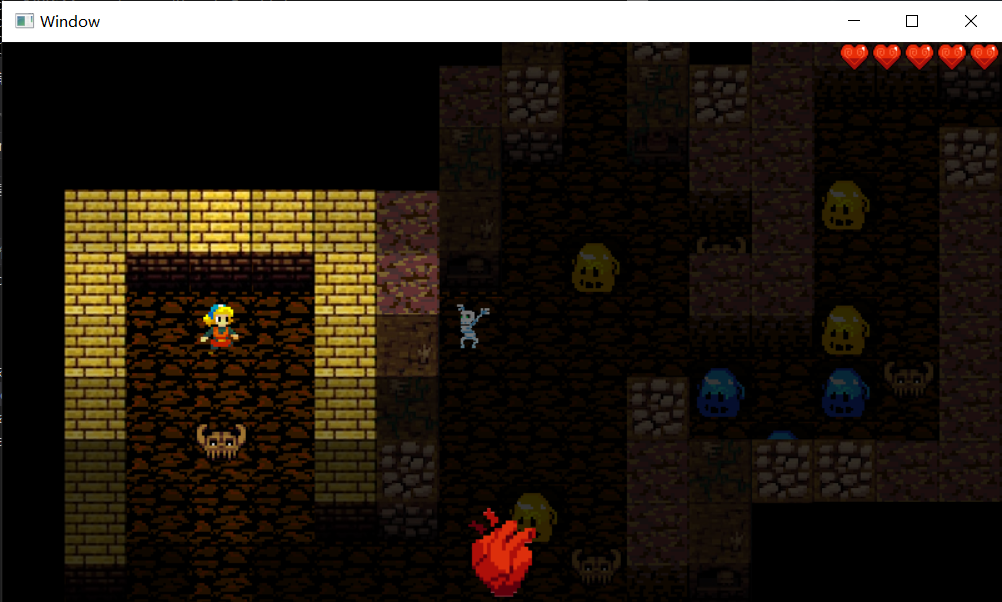
\includegraphics[width=0.95\textwidth]{imgs/1}
\end{figure}
主要使用Gdi进行绘制,所有绘图素材均是BMP
\paragraph{地形}将整个窗口分成16*9个50px*50px的方格,在网格绘制一个50*50的素材即可画出地面;以网格底部线为基准绘制一个50*82的素材即可画出立体墙面。绘图时从上到下逐行绘制,因此下面行绘制的墙可以挡住上面行绘制的素材,达到看上去立体的效果。代码中\_PaintObjectAtPos函数即抽象了在某个网格位置上绘制一个素材的逻辑。
\paragraph{人物、怪物}在绘制某个网格上的地形时,判断该位置上是否有玩家或敌人,有则在该位置额外绘制一个敌人、玩家的贴图,玩家和敌人的贴图是不包含透明信息的50*50的bmp,但却不会挡住该网格的地面贴图,这由TransparentBlt实现
\paragraph{心脏、血量红心}直接计算其在窗口中的绝对坐标并绘制。心脏会在每个节拍上跳动,这通过在对应时间点上将小心脏替换成大心脏再替换回来实现
\paragraph{玩家居中}在玩家移动时,游戏将尽量让玩家居于窗口的中部,这通过将当前绘制的窗口抽象成一个在整个地图上滑动的视窗实现,玩家移动将导致这个视窗和玩家同步移动,因此玩家总位于窗口中心,看上去的效果是地面相对整个窗口移动了。
\paragraph{阴影}离玩家越远,地图越黑暗,且被墙体遮挡的地区是完全黑暗不可见的,这些都是地牢类游戏渲染气氛的常用手段,本项目也近似实现了这些效果。方法是为每个绘制的位置通过其离玩家的距离和被墙体遮挡的程度计算一个alpha值,然后通过AlphaBlend将一个纯黑的Mask按照这个alpha值渲染到绘制位置上,alpha值越高,黑暗程度越重。
\paragraph{避免闪烁}Gdi绘图容易出现闪烁问题,而本项目通过双缓冲完全解决了闪烁。绘图时先创建一个和窗体一样大的缓冲区,再对每个要绘制的贴图创建一个小缓冲区并通过SelectObject将贴图放到小缓冲区中,将贴图从小缓冲区贴到大缓冲区中对应的位置,最后将大缓冲区一次性贴到窗体中(而非每次都把一个小缓冲区贴到窗体中)。
\subsection{音乐与节拍}
音乐通过PlaySound播放。

事先用其他工具计算出节拍间的时间间隔,然后用SetTimer设置计时器,每到节拍的时间点上就触发一次WM\_Timer事件,在这个事件里,将会完成玩家移动、怪物移动、攻击等等游戏相关的状态更新(在updateStatus中实现),上述状态更新完成后,触发InvalidRect以重绘窗口。不过由于Windows的Timer并非精确计时,加上WM\_Timer的优先级较低,因此有时候会出现丢拍,目前没有很好的解决办法。
\subsection{游戏逻辑}
用户的输入会改变玩家的nextStep变量,在每个节拍上触发的updateStatus函数中,按以下逻辑执行
\begin{enumerate}
	\item 通过player.nextStep判断玩家下一步将要去的的位置(nextPos)
	\item 通过checkCollision函数判断nextPos是否可达(有没有墙体、敌人等阻挡),如果可达,前往3.,否则前往4.
	\item (可达)更新玩家的位置为nextPos,清空nextStep。前往5.
	\item (不可达)不更新玩家位置,清空nextStep。判断阻挡玩家的物体类型,如果是可以挖掘的墙壁(土墙),则挖掘之;如果是怪物,则攻击之。前往5.
	\item 遍历敌人列表,对每个还活着的敌人,通过decideNextStep函数,根据敌人的\textbf{移动类型*}计算其nextStep
	\item 通过该敌人的nextStep判断其下一步将要去的位置(nextPos)
	\item 通过checkCollision函数判断nextPos是否可达(有没有墙体、敌人、玩家等阻挡),如果可达,前往6.,否则前往7.
	\item (可达)更新敌人的位置为nextPos,清空nextStep。前往10.
	\item (不可达)不更新敌人位置,清空nextStep。判断阻挡敌人的物体类型,如果是玩家,则攻击之。前往10.
	\item 判断玩家血量和位置,如果位置为陷阱,则将其血量减为0;如果血量为0,则触发游戏结束函数;如果位置为楼梯,则触发游戏胜利函数
	\item 如果游戏没有结束或胜利,则在下一个节拍上重新从1.开始执行
\end{enumerate}
\textbf{*移动类型} \quad 按怪物区分,有以下几种
\begin{itemize}
	\item \textbf{蝙蝠}\quad 2拍动一次,上下左右随机移动
	\item \textbf{蓝色史莱姆}\quad 2拍动一次,上下来回跳动
	\item \textbf{金色史莱姆}\quad 1拍动一次,顺时针转圈跳动
	\item \textbf{骷髅}\quad 2拍动一次,追逐玩家,采用贪心追逐算法
\end{itemize}
\subsection{信息储存}
玩家和敌人用结构体储存,地图用一个一维数组(大小为MAP\_WIDTH*MAP\_HEIGHT)储存,每个位置为一个数字,储存了地形信息
\subsection{资源管理}
程序打开时加载所有资源;程序关闭时删除所有资源。具体逻辑在\_InitResources与\_DestroyResources中实现
\section{难点和创新点}
\subsection{难点}
\begin{enumerate}
	\item 一开始整体上没有一个入门win32编程的教材,且网上资料较少,以至于不知道从何入手。后通过《Windows环境下32位汇编语言程序设计》 (罗云彬著)一书+微软的win32\ api文档入门
	\item 一开始遇到了严重的绘图闪烁问题,后通过双缓冲解决
	\item 节奏需要时间上的严格精确,但Timer无法做到十分精确,所以本游戏最关键的节奏其实实现得不完美(丢拍,错节奏),且至今没有解决,最后修改成了每个节拍怪物都会移动,而玩家也可以在非节拍点上移动
\end{enumerate}
\subsection{创新点}
游戏中阴影的绘制、怪物血量、人物血量、被攻击时的闪屏、跳动的心脏等都可以作为创新点,让这个游戏的完成度显得更高。
\section{小组分工}
\begin{itemize}
	\item \textbf{周雨豪}\quad 组织协调工作;调查win32音频播放方法;实现节奏相关部分和用户输入处理
	\item \textbf{叶宸} \quad 实现主要的游戏逻辑(如updateStatus等);地图设计;敌人设计;文档编写
	\item \textbf{徐源远}\quad 调查win32的绘图方法;实现主要的绘图函数(如\_PaintObject等)
\end{itemize}








\end{document}